\section{Coupling EnergyPlus with Functional Mock-up Units for co-simulation}\label{coupling-energyplus-with-functional-mock-up-units-for-co-simulation}

The Functional Mock-up Unit (FMU) for co-simulation import for EnergyPlus allows EnergyPlus to conduct co-simulation with various programs that are packaged as FMUs. A FMU is a component which implements the Functional Mock-up Interface (FMI) standard (\url{http://www.modelisar.com}).

A FMU is distributed in the form of a zip file that may contain physical models, model descriptions, source code, and executable programs for various platforms. The FMU for co-simulation import provides EnergyPlus with a standard interface to conduct and control co-simulation with an arbitrary number of FMUs without any middle-ware, such as the Building Controls Virtual Test Bed (BCVTB Documentation, 2011).

The FMU for co-simulation import allows coupling of continuous-time and discrete-time models exported from different simulation programs. In the current implementation, EnergyPlus is implemented as the co-simulation master. It controls the data exchange between the subsystems and the synchronization of all slave simulation programs.

The FMU for co-simulation import enables the direct link between the EnergyPlus kernel and other simulation tools. It will make the co-simulation easier to conduct as no middle-ware is involved. This direct link will decrease run-time by eliminating the transaction layer. In addition, by separating the co-simulation interface from the EnergyPlus kernel, the FMU interface is reusable when EnergyPlus is updated. Furthermore, the FMU contains executable files that have the same interface to EnergyPlus regardless of their original programming environment. Some commercial tools allow running their FMU without licensing requirement.

\textbf{Notes:}

1)~~~The current implementation of FMU for co-simulation is only supported on Windows and Linux.

2)~~~FMUs must be in a folder to which the user has \emph{write} access.

\subsection{Data exchange between EnergyPlus and FMUs}\label{data-exchange-between-energyplus-and-fmus}

Prior to describing the data exchange between EnergyPlus and FMUs, some definitions and terminologies used in the remainder of this document will be introduced.

A variable of a system described by a system of differential algebraic equations (DAE) is defined as differential variable if its derivatives are present in the DAE. A variable of a system described by a system of DAE is defined as algebraic if its derivatives do not appear explicitly in the DAE (Fabian et al., 2008).

\begin{figure}[hbtp] % fig 5
\centering
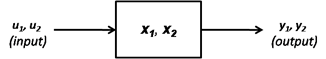
\includegraphics[width=0.9\textwidth, height=0.9\textheight, keepaspectratio=true]{media/image008.png}
\caption{System with two variables that could be either differential or algebraic variables. \protect \label{fig:system-with-two-variables-that-could-be}}
\end{figure}

Because in subsequent discussions, it will be distinguished between algebraic and differential variables, a notation for different system of equations that involve algebraic and differential variables will be introduced. Let \(q\in\mathbf{N}\) , then

\begin{itemize}
\tightlist
\item
  If x\(_{1}\) and x\(_{2}\)~are differential variables, then the system is
\end{itemize}

\(F\left(\dot x_1,x_1,\dot x_2,x_2,u,t\right) = 0\) ~with \emph{F}: ℝ\(^{n}\) x ℝ\(^{n}\) x ℝ\(^{m}\) x ℝ\(^{m}\) x ℝ\(^{q}\) x ℝ → ℝ\(^{n+m}\).

\begin{itemize}
\tightlist
\item
  If x\(_{1}\) is a differential variable and x\(_{2}\)~is an algebraic variable, then the system is
\end{itemize}

\(G\left(\dot x_1,x_1,x_2,u,t\right) = 0\) ~with \emph{G}: ℝ\(^{n}\) x ℝ\(^{n}\) x ℝ\(^{m}\) x ℝ\(^{q}\) x ℝ → ℝ\(^{n+m}\).

\begin{itemize}
\tightlist
\item
  If x\(_{1}\)~is an algebraic variable and x\(_{2}\)~is a differential variable, then the system is
\end{itemize}

\(H\left(x_1,\dot x_2,x_2,u,t\right) = 0\) ~with \emph{H:} ℝ\(^{n}\) xℝ\(^{m}\) xℝ\(^{m}\) xℝ\(^{q}\) xℝ →ℝ\(^{n+m}\).

\begin{itemize}
\tightlist
\item
  If x\(_{1}\)~is an algebraic variable and x\(_{2}\)~is an algebraic variable, then the system is
\end{itemize}

\(I\left(x_1,x_2,u,t\right) = 0\) with \emph{I}: ℝ\(^{n}\) xℝ\(^{m}\) xℝ\(^{q}\) xℝ →ℝ\(^{n+m}\).

Figure~\ref{fig:system-with-one-fmu-linked-to-energyplus.}~shows a case where a FMU is linked to an EnergyPlus model for co-simulation. The FMU and EnergyPlus could be linked through differential or algebraic variables.

\begin{figure}[hbtp] % fig 6
\centering
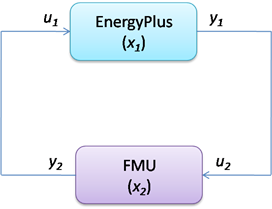
\includegraphics[width=0.9\textwidth, height=0.9\textheight, keepaspectratio=true]{media/image016.png}
\caption{System with one FMU linked to EnergyPlus. \protect \label{fig:system-with-one-fmu-linked-to-energyplus.}}
\end{figure}

Table \ref{table:use-cases-with-different-system-configurations} shows the different system configurations that are possible. 

\begin{itemize}
\item
  In the first case, the variable x\(_{1}\)~and x\(_{2}\)~are differential variables in both systems.
\item
  In the second case, the variable x\(_{1}\)~is a differential variable and the variable x\(_{2}\)~is an algebraic variable.
\item
  In the third case, the variable x\(_{1}\)~is an algebraic variable and the variable x\(_{2}\) is a differential variable.
\item
  In the fourth case, the variable x\(_{1}\)~is an algebraic variable and the variable x\(_{2}\) is an algebraic variable.
\end{itemize}

In the current implementation, it will be focused on the first and the second cases since the third and the fourth cases will constrain the FMU to be solved numerically in the iteration solver loop of EnergyPlus. This will necessitate the ability of the FMU to reject time steps (Modelisar, 2010) which is currently not implemented in the EnergyPlus FMU for co-simulation import. Applications for case 1 and 2 are described in the next sections.

\begin{longtable}[c]{@{}lll@{}}
\caption{Use cases with different system configurations \label{table:use-cases-with-different-system-configurations}} \tabularnewline
\toprule 
Case & EnergyPlus & FMU (e.g. from Modelica) \tabularnewline
\midrule
\endfirsthead

\caption[]{Use cases with different system configurations} \tabularnewline
\toprule 
Case & EnergyPlus & FMU (e.g. from Modelica) \tabularnewline
\midrule
\endhead

(1) & Model1 (Differential variable) & Model2 (Differential variable) \tabularnewline
(2) & Model1 (Differential variable) & Model2 (Algebraic variable) \tabularnewline
(3) & Model1 (Algebraic variable) & Model2 (Differential variable) \tabularnewline
(4) & Model1 (Algebraic variable) & Model2 (Algebraic variable) \tabularnewline
\bottomrule
\end{longtable}

\subsection{Case 1: Linking two systems through differential variables}\label{case-1-linking-two-systems-through-differential-variables}

This case could be for an application where a wall with a phase change material (PCM) is modeled in a FMU and is linked to a room model in EnergyPlus. The room air temperature is the differential variable in EnergyPlus and the temperature of the wall with PCM is the differential variable in the FMU. Each system solves a differential equation that is connected~to the differential equation of the other system. For simplicity, we assume that \emph{y\(_{1}\)(.)} = \emph{x\(_{1}\)(.) and y\(_{2}\)(.)} = \emph{x\(_{2}\)(.).}The systems are described by the ordinary differential equations

dx\(_{1}\)/dt = f\(_{1}\)(x\(_{1}\), x\(_{2}\)), with x\(_{1}\)(0) = x\(_{1,0}\) ,

dx\(_{2}\)/dt = f\(_{2}\)(x\(_{2}\), x\(_{1}\)), with x\(_{2}\)(0) = x\(_{2,0\\ .}\)

Let \(N\in\textbf{N}\) ~denote the number of time steps and let \emph{t\(_{k}\)} with \(k\in\left\{1,...,N\right\}\) denote the time steps. We will use the subscripts \emph{1} and \emph{2} to denote the variables and the functions that compute the next state variable of the simulator \emph{1} and \emph{2}, respectively.

The first system computes, for \(k\in\left\{0,...,N-1\right\}\) and some \(\tilde{F}_1\) : ℝ\(^{n}\) x ℝ\(^{m}\) x ℝ x ℝ → ℝ\(^{n}\), the sequence

x\(_{1}\)(t\(_{k+1}\)) = \(\tilde{F}_1\) (x\(_{1}\)(t\(_{k}\)), x\(_{2}\)(t\(_{k}\)), t\(_{k}\), t\(_{k+1}\))

and, similarly, the simulator \emph{2} computes for some \(\tilde{F}_2\) : ℝ\(^{m}\) x ℝ\(^{n}\) x ℝ x ℝ → ℝ\(^{m}\) the sequence

x\(_{2}\)(t\(_{k+1}\)) = \(\tilde{F}_2\) (x\(_{2}\)(t\(_{k}\)), x\(_{1}\)(t\(_{k}\)), t\(_{k}\), t\(_{k+1}\))

with initial conditions \emph{x\(_{1}\)(0) = x\(_{1,0}\)} and \emph{x\(_{2}\)(0) = x\(_{2,0.}\)} \(\tilde{F}_1\) ~and \(\tilde{F}_2\) ~*are the functions that are used to compute the value of the state variables at the new time step

To advance from time \emph{t\(_{k}\)} to \emph{t\(_{k+1}\)}, each system uses its own time integration algorithm. At the end of the time step, EnergyPlus sends the new state \emph{x\(_{1}\)(t\(_{k+1}\))} to the FMU and it receives the state \emph{x\(_{2}\)(t\(_{k+1}\))} from the FMU. The same procedure is done with the FMU.

\subsection{Case 2: Linking two systems through algebraic and differential variables}\label{case-2-linking-two-systems-through-algebraic-and-differential-variables}

This case could be for an application where a fan is modeled in a FMU and is linked to a room model in EnergyPlus. The room temperature is the differential variable in EnergyPlus and the pressure difference of the fan is the algebraic variable in the FMU. For simplicity, we assume that \emph{y\(_{1}\)(.)} = \emph{x\(_{1}\)(.) and y\(_{2}\)(.)} = \emph{x\(_{2}\)(.).} In this application, the systems are described by the following equations

dx\(_{1}\)/dt = g\(_{1}\)(x\(_{1}\), x\(_{2}\)), with x\(_{1}\)(0) = x\(_{1,0,}\)

0 = g\(_{2}\)(x\(_{2}\), x\(_{1}\)).

Let \(N\in\mathbf{N}\) ~denote the number of time steps and let \emph{t\(_{k}\)} with \(k\in\left\{1,...,N\right\}\) ~denote the time steps. We use the same subscripts \emph{1} and \emph{2} as for the first case to denote the variable and the function that computes the next variable of the simulator \emph{1} and \emph{2}, respectively.

The first system computes, for \(k\in\left\{0,...,N-1\right\}\) and some \(\tilde{G}_1\) : ℝ\(^{n}\) x ℝ\(^{m}\) x ℝ x ℝ → ℝ\(^{n}\), the sequence

x\(_{1}\)(t\(_{k+1}\)) = \(\tilde{G}_1\) (x\(_{1}\)(t\(_{k}\)), x\(_{2}\)(t\(_{k}\)), t\(_{k}\), t\(_{k+1}\))

and, similarly, the simulator \emph{2} computes for some \(\tilde{G}_2\) : ℝ\(^{m}\) x ℝ\(^{n}\) x ℝ → ℝ\(^{m}\) the sequence

x\(_{2}\)(t\(_{k+1}\)) = \(\tilde{G}_2\) (x\(_{2}\)(t\(_{k+1}\)), x\(_{1}\)(t\(_{k+1}\)), t\(_{k+1}\))

with initial condition \emph{x\(_{1}\)(0) = x\(_{1,0}\)}. \(\tilde{G}_1\) and \(\tilde{G}_2\) are the functions that compute the value of the variables at the new time step.

To advance from time \emph{t\(_{k}\)} to \emph{t\(_{k+1}\)}, each system uses its own time integration algorithm. At the end of the time step, EnergyPlus sends the new value \emph{x\(_{1}\)(t\(_{k+1}\))} to the FMU and it receives the value \emph{x\(_{2}\)(t\(_{k+1}\))} from the FMU. The same procedure is done with the FMU.

\subsection{Requirements}\label{requirements}

The current implementation for linking EnergyPlus with the FMUs has the following requirements:

\begin{itemize}
\item
  The data exchange between EnergyPlus and the FMUs is done at the zone time step of EnergyPlus.
\item
  Each FMU is linked to EnergyPlus only through a differential variable in EnergyPlus (see Figure~\ref{fig:system-with-one-fmu-linked-to-energyplus.-001} for one FMU).
\end{itemize}

\begin{figure}[hbtp] % fig 7
\centering
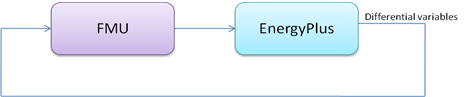
\includegraphics[width=0.9\textwidth, height=0.9\textheight, keepaspectratio=true]{media/image033.png}
\caption{System with one FMU linked to EnergyPlus. \protect \label{fig:system-with-one-fmu-linked-to-energyplus.-001}}
\end{figure}

\begin{itemize}
\tightlist
\item
  Two or multiple FMUs are linked together only through differential variables in EnergyPlus (see Figure~\ref{fig:system-with-two-fmus-linked-to-energyplus.} for two FMUs).
\end{itemize}

\begin{figure}[hbtp] % fig 8
\centering
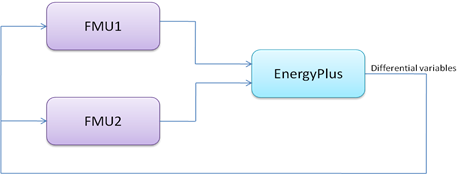
\includegraphics[width=0.9\textwidth, height=0.9\textheight, keepaspectratio=true]{media/image034.png}
\caption{System with two FMUs linked to EnergyPlus. \protect \label{fig:system-with-two-fmus-linked-to-energyplus.}}
\end{figure}
